\chapter{Regionalgeologie}
\authorAnGu
Das Kartiergebiet befindet sich im Rheinischen Schiefergebirge. Dieses ist Teil der Mitteldeutschen variszischen Orogenese. Der Gebirgsbildung vorangestellt ist eine, noch nicht in allen Einzelheiten verstandene Beckenentwicklung, im Devon und Unterkarbon. \cite{franke17}

\Autoref{fig:Kossmat} nun übergeordneten Kontext schlossen sich während der Akkretion Laurussias und Gondwanas, das Rheiische und Rhenoherzynische Becken. Nach der Kossmat'schen Gliederung des deutschen Variszikums, befindet sich das Rheinische Schiefergebirge fast ausschließlich im Rhenoherzynikum, und wird südöstlich durch die nördliche Phyllitzone und das Mitteldeutsche Kritallinhoch begrenzt (siehe \autoref{fig:Kossmat}).

\begin{figure}[!htb]
\centering
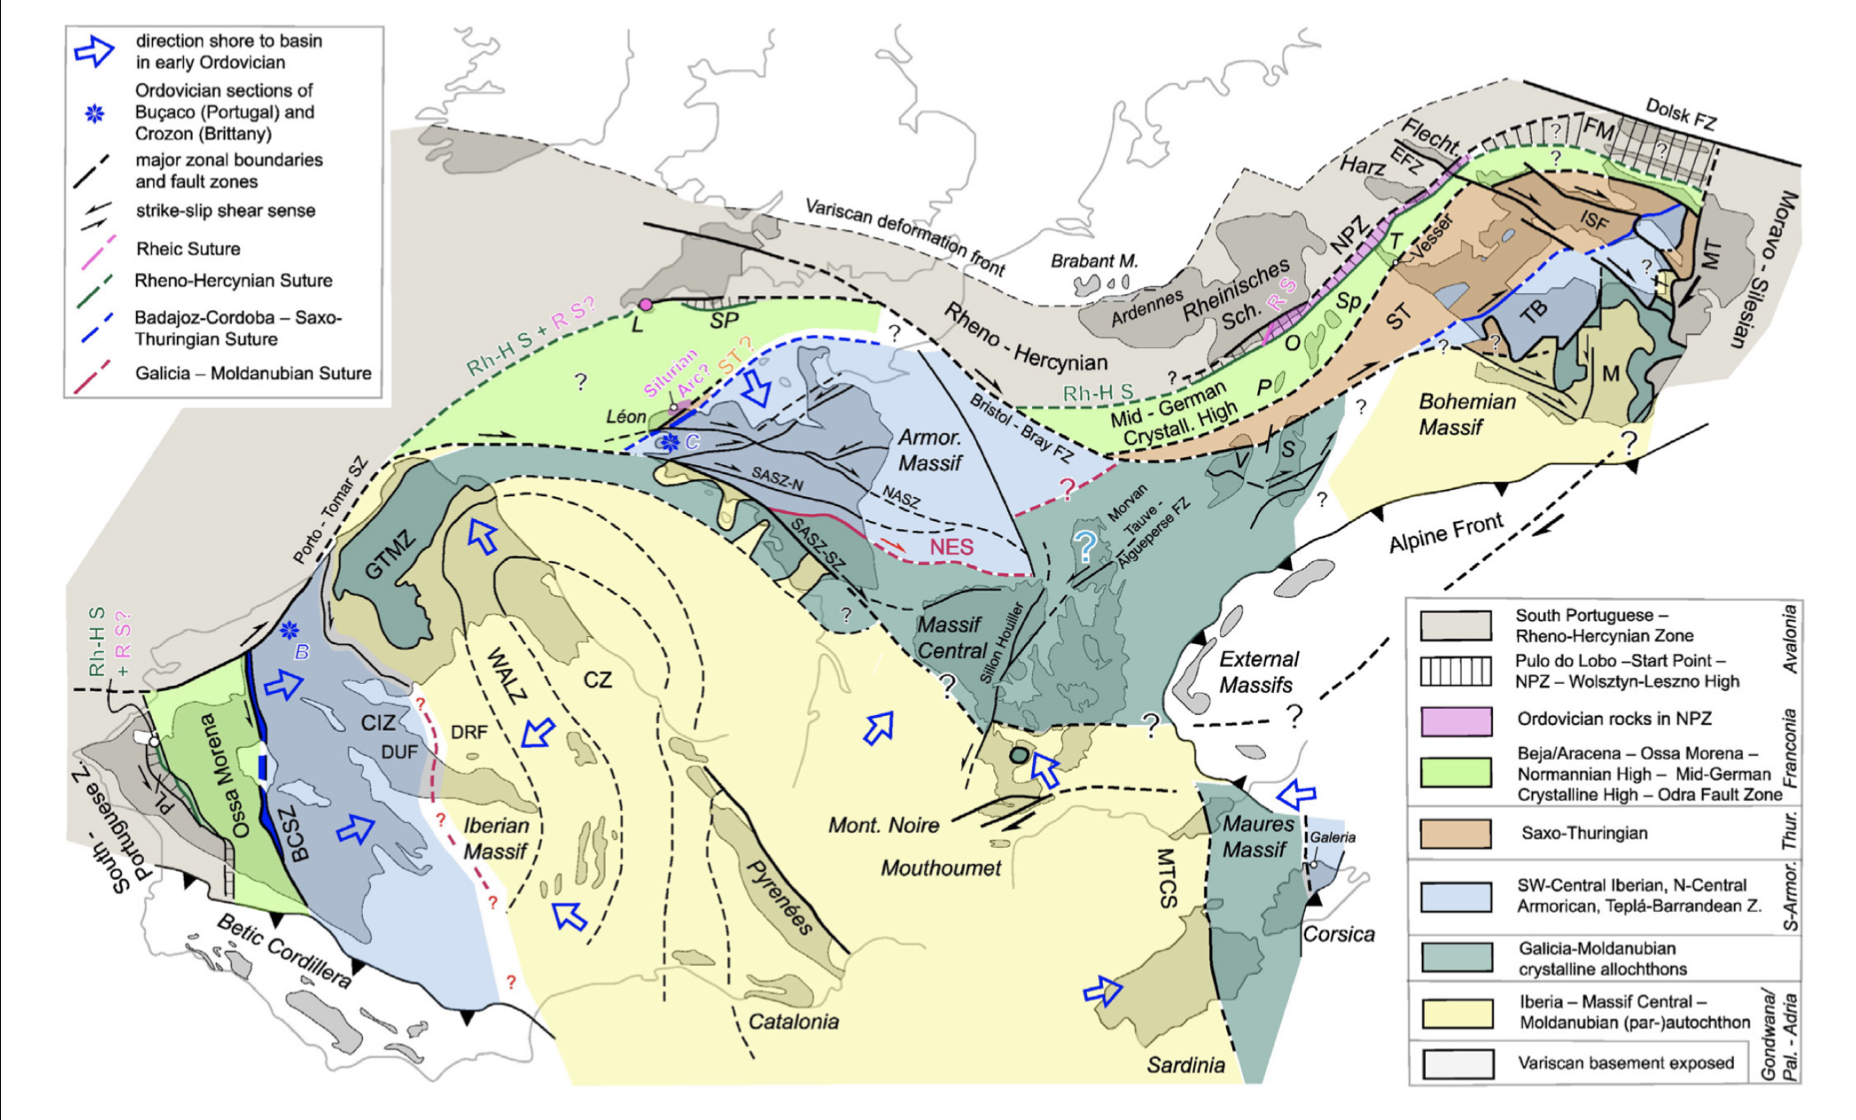
\includegraphics[width=\textwidth]{Ueberblick_Kossmat.png}
\caption{Europäisches Variszikum inklusive Rheinisches Schiefergebirge (\cite{franke17})}
\label{fig:Kossmat}
\end{figure} 

Aus den in \autoref{fig:Kossmat} dargestellten geometrischen Beziehungen folgt:

\begin{equation}
 sin(\alpha)=\frac{\Delta x_1}{\sqrt{(\Delta x_1)^2+s^2}}
 \label{equ:Franke1}
\end{equation}

Für das erste Intensitätsmaximum gilt $n=1$ und somit $\lambda=\Gamma$. $\Gamma$ ist der Gangunterschied. Dieser ist der Wegunterschied  \cite{franke17} zwischen kohärenten Lichtwellen. Abermals gut in \autoref{fig:Styliolin} zu sehen, gilt nun: $sin(\alpha)=\frac{\Gamma}{g}=\frac{\lambda}{g}$. Daraus folgt:
\begin{equation}
\lambda=sin(\alpha)\cdot g
 \label{equ:lambda}
\end{equation}
Und schließlich:
\begin{equation}
\lambda=\frac{\Delta x_1}{\sqrt{(\Delta x_1)^2+s^2}}\cdot g
 \label{equ:lambda1}
\end{equation}


Die zeitliche Abfolge der Beckenschließungen und Kollisionstektonik ist in \autoref{equ:lambda1} abgebildet. Das heutige Rheinische Schiefergebirge befände sich in den Grafiken, stets nördlich des in grün gekennzeichneten Mitteldeutschen Kristallinhochs. Um eine letzte regional-geologische Einordnung vorzunehmen dienen Abbildung. Die Kartiergebiete befinden sich wie in \autoref{equ:lambda} zu sehen, in der Wittgensteiner Mulde, die Proximität zur Lahn- Dillmulde aufweist.  Zeugen dieser Ablagerungsbedingungen sind der Eifelquarzit, Styliolinenschiefer- und Sandsteinfolge, Adorf-Bänderschiefer, Unterer Rotschiefer, Nehden-Sandstein, oberer Rotschiefer, sowie die Dasberg-Schichten \cite{franke17}. 

\cite{Gerth06,kroner07,schwartz08,Brown09,IngGeo11,PhyPro11}

\begin{table}[!h]
\centering
\caption{Messwerte und Ergebnisse}
\label{tab:Laser}
\begin{tabular}{@{}llll@{}}
\toprule
{Messung} & {$\Delta x[cm]$} & {$s[cm]$} & {$\lambda[nm]$} \\ \midrule
rot     & 9,5           & 26    & 689          \\
grün    & 7,3         & 26    & 540          \\ \bottomrule
\end{tabular}
\end{table}

\Autoref{equ:Boole's inequality} am Anfang und soweiter Im Unterdevon kam es zu Transgression und damit einhergehender Hungersedimentation, sowie anschließenden Flyscheintrag, in Folge, der im Südosten einsetzenden Gebirgsbildung. Kulm-Alaunschiefer, Kulm-Kieselschiefer, Kulmtonschiefer, und Kulm-Grauwacken belegen diese. Letztere sind im Kartiergebiet Arfeld jedoch nicht auffindbar. Die Nordwest-Südost gerichtete Einengung hatte intensive nordwest vergente Faltung, sowie Verkürzung der kontinentalen Kruste um 51 Prozent zur Folge. 

\section{Kartiermethodik}

\begin{equation}
P(\bigcup_{n=1}^n A_n) \leq \sum_{n=1}^n P(A_n)
\label{equ:Boole's inequality}
\end{equation}

Where the events $A_n$ are disjoint, then the inequality 
in \autoref{equ:Boole's inequality} becomes an equality.

Die generelle Vorgehensweise bestand darin, die vorkommenden Gesteine anhand lithologischer Merkmale zu identifizieren und senkrecht zum typischen Streichen, das heißt in Richtung Nordwest, oder Südost, zu verfolgen.

\section{Lithologie}

\subsection{Styliolinenschiefer- und Sandstein-Folge (Mitteldevon)}

Es handelt sich hierbei ebenfalls um eine Wechselfolge aus Sand- und Tonsteinen. Die Wechsellagerung ist jedoch regelmäßiger und frequenter. Der Sandstein ist feinsandig, mitunter auch grobsiltig, im großen Unterschied zum Eifelquarzit meist karbonatisch gebunden. Des weiteren sind deutlich Glimmer auf den Schichtflächen erkennbar. Farblich handelt es sich um ein grau braunes Gestein, wobei die hellen Sandsteine sich gut von dunklen Toneinschaltungen abgrenzen lassen. Ein gutes Erkennungsmerkmal sind Styliolinen, konische herausgewitterte Schalenreste, auf den Schichtflächen. Weiterhin ist die Feinlamination wulstig deformiert, und erzeugt so unregelmäßige Bruchstücke. 

\begin{figure}[!htb]
\centering
\includegraphics[width=\textwidth]{Styliolinen}
\caption{Aufschluss 5:,Wulstung der Styliolinenfolge}
\label{fig:Styliolin}
\end{figure} 


\subsection{Nehden-Sandstein (Oberdevon, Nehden)}
Die Sandsteine dieser Folge sind fein- bis mittelsandig, zumeist deutlich grobkörniger als die des Eifelquarzits oder Styliolinensandsteines. Weiterhin sind sie sehr glimmerreich. Bis auf Sohlmarken, die als gute unten-oben Anzeiger dienen, konnten keine Sedimentstrukturen erkannt werden. Pflanzenreste sind bei genauem Betrachten vereinzelt erkennbar. Das Gestein ist sehr kompetent und oft Teil topografischer Positivstrukturen. Die zwischengelagerten Tonsteine sind nicht sehr mächtig, ausnahmslos kleiner als 50 Zentimeter, und sehr dunkel, bis schwarz. Die Sandsteinbänke sind im Kontrast dazu hellgrau. 


\subsection{Dasberg-Schichten (Oberdevon, Dasberg)}

Die Dasbergschichten setzen sich zusammen aus der Hembergschicht and der Basis, gefolgt von der Dasbergfolge, und der Hangenbergschicht am Top. Die Drei Einheiten unterschieden sich jedoch kaum und werden daher zusammen kartiert. Feinsandsteine und Tonsteine sind ähnlich wie in der Styliolinenfolge wechselgelagert. Die Sandsteine sind jedoch durch deutliche Karbonatgehalte gekennzeichnet, sowie durch starke Hellglimmeranreicherung auf den Schichtflächen. Weiterhin ist die Wulstung nochmals deutlicher als im Styliolinensandtsein (\autoref{fig:Styliolin}). Die Sandsteine erscheinen intern knubbelig oder faltig, Rippelstrukturen sind erkennbar aber oft auch von der Wulstung überprägt. Der Tonsteinanteil nimmt von der Basis zum Top zu. 
\cite{hoelting12,eckel14,mesch15,vinx15,MiGe15,Hydrod16,grotzinger17,franke17,eckel14,NaCl2,Gneiss}

